% Provenance (never printed): see sources/outline_sources.md (Year 1: stress and
% principal stresses in 2D; strain; pure and simple shear; elastic, brittle and ductile
% behaviour; the strength envelope of the lithosphere). Strength envelopes from
% figdata/bachelor-1/strength_envelope.py (Byerlee 1975; flow laws of Gleason and Tullis
% 1995 and Hirth and Kohlstedt 2003 as compiled by Lopez-Sanchez; geotherms of ch. 10);
% exercise and problem values in the Book 3 scratch calculator calc/ch16.py. Traction,
% shear stress, the stress and strain tensors, Hooke's law, Young's modulus and viscosity
% belong to the physics series and are recalled, never defined (sync 1 ruling).
\chapter{Stress, Strain and Rheology}\label{ch:b1:stress-strain-rheology}

In the 1960s, waste fluid pumped down a disposal well at the Rocky Mountain
Arsenal, near Denver, spread through fractured crystalline basement between
\qty{3.7}{km} and \qty{7.0}{km} below the surface, and earthquakes followed.
They stayed inside the part of the rock where the fluid pressure had risen by
more than about \qty{3.2}{MPa}.
% ledger: hb81:denver
Half a century later the same thing happened on a larger scale in Oklahoma,
where salty water brought up with oil and gas is pumped back underground. In
and around the state, the earthquakes of magnitude 3 or more numbered one to
five a year from 2005 to 2008, then \num{20} in 2009, \num{585} in 2014 and
\num{888} in 2015, more than two a day; shocks of magnitude 5.7 and 5.8 shook
Prague, in 2011, and Pawnee, in 2016. Four high-volume disposal wells alone
could account for a fifth of the earthquakes of the central United States, and
set off some more than \qty{30}{km} away.
% ledger: usgs:oklahoma-rate, usgs:prague-pawnee, keranen:oklahoma
The water pushed nothing aside; it only raised the pressure
of the fluid in the pores of the rock. Why should that make a fault slip?
The answer needs three ideas, which are the subject of this chapter: the
stress on a plane inside a rock, the condition under which the plane gives
way, and the fact that the pressure of the pore fluid counts against the
force pressing the two sides together. With them, and with a law of creep for
hot rock, we can draw the strength of the whole \omterm{def:b1:layered-earth:lithosphere}{lithosphere} against depth.

\begin{recall}
A force spread over a surface acts through its force per unit area, in pascals;
the pressure in a fluid at rest grows with depth as $\rho g z$ (physics books).
A spring, and a solid in small deformations, obey Hooke's law: the strain is
proportional to the stress, with Young's modulus as the constant; a viscous
fluid resists in proportion to its rate of shear, with its viscosity as the
constant. The physics books' University Year 3 volume describes stress and
strain in three dimensions with tensors; this chapter needs only two. A
symmetric $2\times2$ matrix has two real eigenvalues and two perpendicular
eigenvectors (mathematics, Year 1). The \omterm{def:b1:heat-budget:geotherm}{geotherms} of
\cref{ch:b1:heat-budget} give the temperature at depth; faults were met in
Book 1, grade 7.
\end{recall}

\section{Stress in two dimensions}\label{sec:b1:stress-strain-rheology:stress}

Cut a rock in thought along a small flat surface. The rock on one side presses
on the rock on the other with a force, and the force per unit area is the
traction on that surface, in the physics books' word. Its direction is not, in
general, the direction of the normal to the surface.

\begin{definition}[Normal stress]\label{def:b1:stress-strain-rheology:stress}
On a plane through a point of a rock, the force per unit area that the rock on
one side exerts on the other has a component along the normal to the plane,
the \emph{normal stress}\index{normal stress} $\sigma_n$, and a component
along the plane, the shear stress $\tau$. In the Earth sciences the normal
stress is counted positive when it compresses.
\end{definition}

The sign convention is the opposite of the engineer's. It is chosen because
nearly every stress in the solid Earth is a compression: the weight of the
rock above presses on everything below it.

We work in a vertical plane, with an axis $x$ horizontal and an axis $y$. On a
plane perpendicular to $x$ the \omterm{def:b1:stress-strain-rheology:stress}{normal stress} is $\sigma_{xx}$ and the shear
stress $\sigma_{xy}$; on a plane perpendicular to $y$ they are $\sigma_{yy}$
and $\sigma_{yx}$. The two shear stresses are equal: on a small square, the
shear forces on the vertical sides make a couple of moment
$\sigma_{xy}a\cdot a$ for a side $a$, those on the horizontal sides a couple
$\sigma_{yx}a\cdot a$ turning the other way, and the square would spin if
they differed. So three numbers describe the stress at a point, and they are
enough to give it on every plane.

\begin{proposition}[Stress on an inclined plane]\label{prop:b1:stress-strain-rheology:transformation}
Let a plane have the unit normal $\vec n = (\cos\theta, \sin\theta)$, at the
angle $\theta$ from the axis $x$, and let $\vec m = (-\sin\theta, \cos\theta)$
be the unit vector along the plane. The normal and shear stresses on it are
\begin{align*}
  \sigma_n &= \sigma_{xx}\cos^2\theta + 2\sigma_{xy}\sin\theta\cos\theta + \sigma_{yy}\sin^2\theta
           = \frac{\sigma_{xx}+\sigma_{yy}}{2} + \frac{\sigma_{xx}-\sigma_{yy}}{2}\cos2\theta + \sigma_{xy}\sin2\theta, \\
  \tau     &= (\sigma_{yy}-\sigma_{xx})\sin\theta\cos\theta + \sigma_{xy}(\cos^2\theta - \sin^2\theta)
           = -\frac{\sigma_{xx}-\sigma_{yy}}{2}\sin2\theta + \sigma_{xy}\cos2\theta ,
\end{align*}
with $\tau$ counted positive along $\vec m$.
\end{proposition}

\begin{proof}
Cut out a small prism, as in the figure below: an
inclined face of area $A$ with the outward normal $\vec n$, a vertical face of
area $A\cos\theta$ and a horizontal face of area $A\sin\theta$, per unit
length in the third direction. Its weight and its inertia scale as its volume,
which shrinks faster than its faces; for a small enough prism the forces on
the faces must balance on their own. Compression being positive, the rock
outside pushes on the vertical face with the force
$A\cos\theta\,(\sigma_{xx}, \sigma_{xy})$ and on the horizontal face with
$A\sin\theta\,(\sigma_{xy}, \sigma_{yy})$; on the inclined face it pushes
with $-A(\sigma_n\vec n + \tau\vec m)$. The sum is zero:
\[
  \sigma_n\vec n + \tau\vec m = \cos\theta\,(\sigma_{xx}, \sigma_{xy}) + \sin\theta\,(\sigma_{xy}, \sigma_{yy}) .
\]
The scalar product with $\vec n$ gives $\sigma_n$, with $\vec m$ gives $\tau$,
since $\vec n\cdot\vec m = 0$. The second forms follow from
$\cos^2\theta = (1+\cos2\theta)/2$, $\sin^2\theta = (1-\cos2\theta)/2$ and
$2\sin\theta\cos\theta = \sin2\theta$.
\end{proof}

\begin{omfigure}
\begin{tikzpicture}[>={Stealth[length=5pt]}, font=\small]
% theta = 35 deg, hypotenuse L = 4.5: a = L cos(theta), b = L sin(theta)
\pgfmathsetmacro{\th}{35}
\pgfmathsetmacro{\L}{4.5}
\pgfmathsetmacro{\a}{\L*cos(\th)}
\pgfmathsetmacro{\b}{\L*sin(\th)}
\coordinate (O) at (0,0);
\coordinate (A) at (0,\a);
\coordinate (B) at (\b,0);
\coordinate (M) at ($(A)!0.5!(B)$);
\fill[omLithGranite!45] (O) -- (A) -- (B) -- cycle;
\draw[line width=0.8pt] (O) -- (A) -- (B) -- cycle;
% axes
\draw[->, black!70] (-2.6,-1.9) -- (-1.6,-1.9) node[right] {$x$};
\draw[->, black!70] (-2.6,-1.9) -- (-2.6,-0.9) node[above] {$y$};
% face on x = 0 (outward normal -x), area A cos(theta)
\draw[->, line width=1.1pt, omDef] (-1.35,0.5*\a) -- (-0.05,0.5*\a);
\node[omDef, anchor=south] at (-0.95,0.5*\a+0.05) {$\sigma_{xx} A\cos\theta$};
\draw[->, line width=1.1pt, omProp] (-0.25,0.5*\a-1.25) -- (-0.25,0.5*\a-0.25);
\node[omProp, anchor=east] at (-0.3,0.5*\a-0.85) {$\sigma_{xy} A\cos\theta$};
% face on y = 0 (outward normal -y), area A sin(theta)
\draw[->, line width=1.1pt, omDef] (0.68*\b,-1.35) -- (0.68*\b,-0.05);
\node[omDef, anchor=west] at (0.68*\b+0.05,-1.05) {$\sigma_{yy} A\sin\theta$};
\draw[->, line width=1.1pt, omProp] (0.1,-0.25) -- (1.1,-0.25);
\node[omProp, anchor=north east] at (0.9,-0.32) {$\sigma_{xy} A\sin\theta$};
% inclined face, area A, normal n = (cos theta, sin theta)
\draw[->, line width=1.1pt, omThm] ($(M)+(\th:1.5)$) -- ($(M)+(\th:0.05)$);
\node[omThm, anchor=south west, inner sep=1pt] at ($(M)+(\th:1.5)$) {$\sigma_n A$};
\draw[->, line width=1.1pt, omThm!70!black] ($(M)+(\th:0.25)+(\th-90:0.75)$) -- ($(M)+(\th:0.25)+(\th-90:1.75)$);
\node[omThm!70!black, anchor=west] at ($(M)+(\th:0.3)+(\th-90:1.3)$) {$\tau A$};
\draw[->, black!70, dashed] ($(M)+(\th+90:1.25)$) -- ++(\th:1.0) node[pos=1, anchor=south west, inner sep=1pt, text=black] {$\boldsymbol n$};
% angle theta at A, between the face and the y axis
\pic[draw, angle radius=0.75cm, pic text={$\theta$}, angle eccentricity=1.35] {angle = O--A--B};
\end{tikzpicture}
\par\smallskip{\small The balance of forces on a small triangular prism of
rock. The inclined face has the area $A$ and the unit normal $\vec n$; the
vertical and horizontal faces have the areas $A\cos\theta$ and $A\sin\theta$.
Blue: the normal forces on the two small faces; orange: the shear forces on
them; red: the normal and shear forces on the inclined face. Compression is
counted positive, so every normal force points into the prism.}
\label{fig:b1:stress-strain-rheology:prism}
\end{omfigure}

\begin{theorem}[Principal stresses]\label{thm:b1:stress-strain-rheology:principal}
At every point of a rock there are two perpendicular planes on which the shear
stress is zero. The normal stresses on them are the largest and the smallest
\omterm{def:b1:stress-strain-rheology:stress}{normal stress} over all planes through the point,
\[
  \sigma_{1,3} = \frac{\sigma_{xx}+\sigma_{yy}}{2} \pm
  \sqrt{\Bigl(\frac{\sigma_{xx}-\sigma_{yy}}{2}\Bigr)^2 + \sigma_{xy}^2},
  \qquad \tan2\theta_p = \frac{2\sigma_{xy}}{\sigma_{xx}-\sigma_{yy}},
\]
where $\theta_p$ is the angle from the axis $x$ to the normal of the plane
that carries $\sigma_1$.
\end{theorem}

\begin{proof}
Write $c = (\sigma_{xx}+\sigma_{yy})/2$, and choose $R \ge 0$ and $\theta_p$
with $(\sigma_{xx}-\sigma_{yy})/2 = R\cos2\theta_p$ and
$\sigma_{xy} = R\sin2\theta_p$; then
$R = \sqrt{((\sigma_{xx}-\sigma_{yy})/2)^2 + \sigma_{xy}^2}$ and
$\tan2\theta_p$ is as stated. The second forms of
\cref{prop:b1:stress-strain-rheology:transformation} become
\[
  \sigma_n = c + R\cos(2\theta - 2\theta_p), \qquad \tau = -R\sin(2\theta - 2\theta_p).
\]
The \omterm{def:b1:stress-strain-rheology:stress}{normal stress} is largest, $c + R$, for $\theta = \theta_p$, and smallest,
$c - R$, for $\theta = \theta_p + \ang{90}$; at both, $\tau = 0$. Note also
that $\mathrm d\sigma_n/\mathrm d\theta = 2\tau$: the \omterm{def:b1:stress-strain-rheology:stress}{normal stress} is
stationary exactly where the shear stress vanishes.
\end{proof}

\begin{definition}[Principal stresses, differential stress]\label{def:b1:stress-strain-rheology:principal}
The \emph{principal stresses}\index{principal stresses} at a point are the
normal stresses $\sigma_1 \ge \sigma_3$ on the two planes free of shear
stress, and their directions are the principal directions. In three
dimensions there are three, $\sigma_1 \ge \sigma_2 \ge \sigma_3$, on three
perpendicular planes. The \emph{differential stress}\index{differential
stress} is $\sigma_1 - \sigma_3$, and the mean stress in the plane is
$(\sigma_1+\sigma_3)/2$.
\end{definition}

A state of stress is easiest to read in its principal directions. If we
measure the angle $\theta$ from the direction of $\sigma_1$ instead of from
the axis $x$, the formulas lose their last terms.

\begin{proposition}[Mohr's circle]\label{prop:b1:stress-strain-rheology:mohr}
On a plane whose normal makes the angle $\theta$ with the direction of
$\sigma_1$,
\[
  \sigma_n = \frac{\sigma_1+\sigma_3}{2} + \frac{\sigma_1-\sigma_3}{2}\cos2\theta,
  \qquad
  |\tau| = \frac{\sigma_1-\sigma_3}{2}\,|\sin2\theta| .
\]
As $\theta$ turns, the point $(\sigma_n, |\tau|)$ runs over the upper half of
the circle of centre $((\sigma_1+\sigma_3)/2,\, 0)$ and radius
$(\sigma_1-\sigma_3)/2$, at the angle $2\theta$ from its $\sigma_1$ end. The
largest shear stress, $(\sigma_1-\sigma_3)/2$, acts on the planes at
\ang{45} to the principal directions.
\end{proposition}

\begin{proof}
In the principal axes $\sigma_{xx} = \sigma_1$, $\sigma_{yy} = \sigma_3$ and
$\sigma_{xy} = 0$, and \cref{prop:b1:stress-strain-rheology:transformation}
gives the two formulas. Then
$(\sigma_n - (\sigma_1+\sigma_3)/2)^2 + \tau^2 = ((\sigma_1-\sigma_3)/2)^2$, the
equation of the circle; $|\sin2\theta|$ is largest for $\theta = \ang{45}$.
\end{proof}

The sign of $\tau$ only says in which sense the two sides would slide, so the
upper half of the circle is usually drawn alone. The construction is named
after the engineer Christian Otto Mohr, who also built on it a criterion of
failure, which is where we are going
(\cref{sec:b1:stress-strain-rheology:rheology}).

\subsection*{Stress at depth}

\begin{definition}[Lithostatic pressure, pore-fluid pressure, effective stress]\label{def:b1:stress-strain-rheology:lithostatic}
At the depth $z$, the weight of the rock above, per unit of horizontal area,
is the vertical stress $\sigma_v = \int_0^z\rho g\,\mathrm dz'$, which is
$\rho g z$ in a layer of uniform density $\rho$. When the stress is the same
in every direction and equal to it, the rock is under the \emph{lithostatic
pressure}\index{lithostatic pressure}. The pressure of the water, oil or gas
in the pores and cracks of the rock is the \emph{pore-fluid
pressure}\index{pore-fluid pressure} $P$; it is hydrostatic,
$P = \rho_w g z$, when the pores connect to the surface. The
\emph{effective stress}\index{effective stress} is the stress minus the pore
pressure, $\sigma' = \sigma - P$, on every plane; $\lambda = P/\sigma_v$ is the
pore-pressure ratio.
\end{definition}

In a \omterm{def:b1:layered-earth:layers}{crust} of density \qty{2700}{kg.m^{-3}}, the vertical stress grows by
$2700\times9.81\times1000 = \qty{26.5}{MPa}$ per kilometre and a hydrostatic
pore pressure by \qty{9.81}{MPa} per kilometre: $\lambda = 1000/2700 = 0.37$.
The pore fluid pushes the grains apart with the same pressure in every
direction; it takes nothing from the shear stress, but it takes $P$ from every
\omterm{def:b1:stress-strain-rheology:stress}{normal stress}. Where the pores are sealed, by clay or salt for instance, the
fluid can carry part of the weight of the rock above, and $\lambda$ rises
towards 1.

The stress in the \omterm{def:b1:layered-earth:layers}{crust} is not lithostatic. Plates push and pull, the \omterm{def:b1:layered-earth:layers}{crust}
bends, mountains weigh on their roots, and the horizontal stresses differ from
the vertical one. Near the surface, which carries no shear stress, one
principal direction is vertical, as \cref{ch:b1:faults-folds-fabrics} shows:
$\sigma_v$ is $\sigma_1$, $\sigma_2$ or $\sigma_3$, and the three cases are
the three ways faults move.

\section{Strain}\label{sec:b1:stress-strain-rheology:strain}

Stress is a cause; strain is what the rock records. A fossil drawn out, a
pebble flattened, a bed shortened into \omterm{def:b1:geological-maps:fold}{folds} all measure a change of shape.

\begin{definition}[Extension, stretch, shear strain]\label{def:b1:stress-strain-rheology:strain}
A line of material of length $\ell_0$ deformed to the length $\ell$ has the
\emph{extension}\index{extension (strain)} $e = (\ell - \ell_0)/\ell_0$ and
the \emph{stretch}\index{stretch} $S = \ell/\ell_0 = 1 + e$; a shortening is
a negative extension, a stretch below 1. Two lines of material that were
perpendicular and now make the angle $\ang{90} - \psi$ have been sheared by
the angle $\psi$, and the \emph{shear strain}\index{shear strain} is
$\gamma = \tan\psi$.
\end{definition}

A strain is homogeneous when every small region of the rock deforms in the
same way. The new position $\vec x'$ of the point $\vec x$ is then a linear
function, $\vec x' = F\vec x$, with a constant $2\times2$ matrix $F$ (and
$\det F > 0$, since rock does not turn inside out). Straight lines stay
straight and parallel lines parallel; a square becomes a parallelogram, and a
circle becomes an ellipse.

\begin{proposition}[The strain ellipse]\label{prop:b1:stress-strain-rheology:ellipse}
Under the homogeneous strain $\vec x' = F\vec x$, the circle of radius 1
becomes an ellipse whose semi-axes are the square roots $S_1 \ge S_2$ of the
eigenvalues of $FF^{\mathsf T}$, along its perpendicular eigenvectors. $S_1$
and $S_2$ are the largest and smallest \omterm{def:b1:stress-strain-rheology:strain}{stretches} of all lines of material,
and the area is multiplied by $\det F = S_1S_2$.
\end{proposition}

\begin{proof}
The point $\vec x = F\vec u$ comes from a point $\vec u$ of the circle,
$|\vec u| = 1$, so $|F^{-1}\vec x|^2 = 1$, that is
$\vec x^{\mathsf T}(FF^{\mathsf T})^{-1}\vec x = 1$. The matrix
$B = FF^{\mathsf T}$ is symmetric with positive eigenvalues $\lambda_1 \ge
\lambda_2$ ($\vec v^{\mathsf T}B\vec v = |F^{\mathsf T}\vec v|^2 > 0$); in its
perpendicular eigenvectors the equation reads
$x_1^2/\lambda_1 + x_2^2/\lambda_2 = 1$, an ellipse of semi-axes
$\sqrt{\lambda_1}$ and $\sqrt{\lambda_2}$. A line of material along the unit
vector $\vec u$ has the \omterm{def:b1:stress-strain-rheology:strain}{stretch} $|F\vec u|$, and
$|F\vec u|^2 = \vec u^{\mathsf T}F^{\mathsf T}F\vec u$ lies between the
eigenvalues of $F^{\mathsf T}F$, which are those of $FF^{\mathsf T}$. Finally
$\lambda_1\lambda_2 = \det B = (\det F)^2$.
\end{proof}

\begin{definition}[Strain ellipse]\label{def:b1:stress-strain-rheology:strain-ellipse}
The \emph{strain ellipse}\index{strain ellipse} is the ellipse into which a
homogeneous strain turns a circle of radius 1; its semi-axes are the
principal \omterm{def:b1:stress-strain-rheology:strain}{stretches} $S_1 \ge S_2$, and its axes the principal directions of
the strain.
\end{definition}

Two strains that change the shape of a body equally can be very different.

\begin{definition}[Pure shear, simple shear]\label{def:b1:stress-strain-rheology:shear-types}
A \emph{pure shear}\index{pure shear} is a homogeneous strain that keeps the
area and keeps its principal directions fixed in the rock:
$F = \begin{pmatrix} k & 0 \\ 0 & 1/k\end{pmatrix}$ in those axes, with
$k > 1$. A \emph{simple shear}\index{simple shear} moves every point parallel
to one direction, the shear direction, by $\gamma$ times its distance from a
fixed plane parallel to it:
$F = \begin{pmatrix} 1 & \gamma \\ 0 & 1\end{pmatrix}$.
\end{definition}

Both keep the area, since both determinants are 1. In \omterm{def:b1:stress-strain-rheology:shear-types}{pure shear} the lines of
material along the axes of the \omterm{def:b1:stress-strain-rheology:strain-ellipse}{strain ellipse} are the same lines at every
stage: the strain is coaxial. In \omterm{def:b1:stress-strain-rheology:shear-types}{simple shear} they are not, as the next
proposition and the figure after it show.

\begin{proposition}[The ellipse of simple shear]\label{prop:b1:stress-strain-rheology:simple-shear}
A \omterm{def:b1:stress-strain-rheology:shear-types}{simple shear} $\gamma$ has the principal \omterm{def:b1:stress-strain-rheology:strain}{stretches}
\[
  S_{1,2} = \sqrt{1 + \gamma^2/4} \pm \gamma/2 ,
\]
and the long axis of its \omterm{def:b1:stress-strain-rheology:strain-ellipse}{strain ellipse} makes with the shear direction the
angle $\theta'$ given by $\tan2\theta' = 2/\gamma$.
\end{proposition}

\begin{proof}
$FF^{\mathsf T} = \begin{pmatrix} 1+\gamma^2 & \gamma \\ \gamma & 1\end{pmatrix}$
has the trace $2+\gamma^2$ and the determinant 1. So $S_1S_2 = 1$ and
$S_1^2 + S_2^2 = 2 + \gamma^2$, hence $(S_1 - S_2)^2 = \gamma^2$,
$S_1 - S_2 = \gamma$, and $S_1 = \gamma/2 + \sqrt{1+\gamma^2/4}$. The
eigenvector of the largest eigenvalue of a symmetric matrix
$\begin{pmatrix} a & b \\ b & d\end{pmatrix}$ makes with the first axis the
angle given by $\tan2\theta' = 2b/(a-d)$ (\cref{thm:b1:stress-strain-rheology:principal}
is the same computation): here $2\gamma/\gamma^2 = 2/\gamma$.
\end{proof}

\begin{omfigure}
\begin{tikzpicture}[>={Stealth[length=4.5pt]}, font=\small, scale=0.95]
% unit square [-1,1]^2 with its inscribed circle, mapped by exact linear maps (cm = a,b,c,d: x' = a x + c y, y' = b x + d y)
% pure shear: diag(k, 1/k), k = (1 + sqrt 5)/2 = 1.618; simple shear: gamma = 1, S1 = 1.618, long axis at 31.72 deg
\pgfmathsetmacro{\k}{(1+sqrt(5))/2}
\pgfmathsetmacro{\ik}{1/\k}
% (a) undeformed
\begin{scope}
  \fill[omLithSand!70] (-1,-1) rectangle (1,1);
  \draw[line width=0.7pt] (-1,-1) rectangle (1,1);
  \draw[line width=0.9pt, omDef] (0,0) circle[radius=1];
  \draw[omThm, line width=0.6pt] (-1,-1) -- (1,1);
  \draw[omProp, line width=0.6pt] (-1,1) -- (1,-1);
  \node[font=\small\bfseries] at (0,-1.55) {(a) before};
\end{scope}
% (b) pure shear
\begin{scope}[xshift=4.2cm]
  \draw[black!35, dashed] (-1,-1) rectangle (1,1);
  \begin{scope}[cm={\k,0,0,\ik,(0,0)}]
    \fill[omLithSand!70] (-1,-1) rectangle (1,1);
    \draw[line width=0.7pt] (-1,-1) rectangle (1,1);
    \draw[line width=0.9pt, omDef] (0,0) circle[radius=1];
    \draw[omThm, line width=0.6pt] (-1,-1) -- (1,1);
    \draw[omProp, line width=0.6pt] (-1,1) -- (1,-1);
  \end{scope}
  \draw[omDef, dashed] (-\k,0) -- (\k,0);
  \draw[omDef, dashed] (0,-\ik) -- (0,\ik);
  \draw[->, line width=0.8pt] (1.72,0) -- (2.15,0);
  \draw[->, line width=0.8pt] (-1.72,0) -- (-2.15,0);
  \draw[->, line width=0.8pt] (0,1.2) -- (0,0.72);
  \draw[->, line width=0.8pt] (0,-1.2) -- (0,-0.72);
  \node[font=\small\bfseries] at (0,-1.55) {(b) pure shear};
\end{scope}
% (c) simple shear, gamma = 1
\begin{scope}[xshift=9.0cm]
  \draw[black!35, dashed] (-1,-1) rectangle (1,1);
  \begin{scope}[cm={1,0,1,1,(0,0)}]
    \fill[omLithSand!70] (-1,-1) rectangle (1,1);
    \draw[line width=0.7pt] (-1,-1) rectangle (1,1);
    \draw[line width=0.9pt, omDef] (0,0) circle[radius=1];
    \draw[omThm, line width=0.6pt] (-1,-1) -- (1,1);
    \draw[omProp, line width=0.6pt] (-1,1) -- (1,-1);
  \end{scope}
  % long and short axes of the strain ellipse: S1 = 1.618 at 31.72 deg, S2 = 0.618 at 121.72 deg
  \draw[omDef, dashed] (211.72:\k) -- (31.72:\k);
  \draw[omDef, dashed] (121.72:\ik) -- (301.72:\ik);
  \draw[->, line width=0.8pt] (-1.2,1.3) -- (0.8,1.3);
  \draw[->, line width=0.8pt] (1.2,-1.3) -- (-0.8,-1.3);
  \draw[black!60] (-2,-1) -- (-2,0.2);
  \draw[black!70] (-2,-0.3) arc[start angle=90, end angle=45, radius=0.7];
  \node[font=\scriptsize] at ($(-2,-1)+(67.5:0.98)$) {$\psi$};
  \node[font=\small\bfseries] at (0,-1.75) {(c) simple shear};
\end{scope}
\end{tikzpicture}
\par\smallskip{\small A square of rock with its inscribed circle (a), deformed
by a \omterm{def:b1:stress-strain-rheology:shear-types}{pure shear} with $k = 1.618$ (b) and by a \omterm{def:b1:stress-strain-rheology:shear-types}{simple shear} with $\gamma = 1$
(c), which has the same principal \omterm{def:b1:stress-strain-rheology:strain}{stretches}, 1.618 and 0.618. Dashed blue:
the axes of the \omterm{def:b1:stress-strain-rheology:strain-ellipse}{strain ellipse}; dashed grey: the square before. In \omterm{def:b1:stress-strain-rheology:shear-types}{pure shear}
the axes stay on the same lines of material; in \omterm{def:b1:stress-strain-rheology:shear-types}{simple shear} the long axis
lies at \ang{31.7} to the shear direction, and the diagonal that was the
direction of fastest stretching at the start (red) has already turned past
it, to \ang{26.6}. The shapes are exact images of the square and the circle
under the two matrices.}
\label{fig:b1:stress-strain-rheology:shear}
\end{omfigure}

The \omterm{def:b1:stress-strain-rheology:strain-ellipse}{strain ellipse} records the total, or \emph{finite}, strain. A deformation
that goes on for millions of years is the sum of many small increments, each
an infinitesimal strain; for a small $\gamma$ the proposition gives
$S_{1,2} \approx 1 \pm \gamma/2$ and $\theta' \approx \ang{45}$. In \omterm{def:b1:stress-strain-rheology:shear-types}{simple
shear} the increments always \omterm{def:b1:stress-strain-rheology:strain}{stretch} fastest at \ang{45} to the shear
direction, while the finite ellipse turns towards it, \ang{31.7} at
$\gamma = 1$, \ang{22.5} at $\gamma = 2$, ever closer as $\gamma$ grows. This
is why flattened pebbles and stretched \omterm{def:b1:rock-forming-minerals:mineral}{minerals} in a zone of intense shear lie
almost in its plane, and why the angle they make with the zone measures how
far it has moved.

\section{Rheology}\label{sec:b1:stress-strain-rheology:rheology}

\begin{definition}[Rheology, brittle and ductile behaviour]\label{def:b1:stress-strain-rheology:rheology}
The \emph{rheology}\index{rheology} of a material is the way it deforms and
flows under stress: the relation between stress, strain and the rate of
strain. A rock shows \emph{brittle behaviour}\index{brittle behaviour} when
it deforms by fracture or by sliding on fractures, on discrete surfaces, with
a sudden loss of strength; it shows \emph{ductile behaviour}\index{ductile
behaviour} when it deforms permanently and continuously through its volume,
without losing its \omterm{def:b1:stress-strain-rheology:coulomb}{cohesion}.
\end{definition}

Rocks show all the behaviours of the physics books. Under small, brief
stresses they are elastic: the strain is proportional to the stress, as in
Hooke's law, and disappears with it; seismic waves
(\cref{ch:b1:layered-earth}) travel through elastic rock. Over long times the
hot \omterm{def:b1:layered-earth:layers}{mantle} flows like a very viscous fluid, the strain rate growing with the
stress. In between, cold rock breaks and slides, and warm rock creeps. Which
behaviour wins depends on the stress, the temperature, the pressure, the fluid
in the pores and the time allowed.

\subsection*{Brittle failure}

\begin{definition}[Coulomb failure criterion]\label{def:b1:stress-strain-rheology:coulomb}
A rock obeys the \emph{Coulomb failure criterion}\index{Coulomb failure
criterion} if a plane through it breaks, or an existing fracture slips, as
soon as on that plane
\[
  \tau = C + \mu\,\sigma_n' , \qquad \sigma_n' = \sigma_n - P ,
\]
where $C \ge 0$ is the \emph{cohesion}\index{cohesion} of the rock,
$\mu$ its \emph{coefficient of internal friction}\index{coefficient of
internal friction} and $\phi = \arctan\mu$ its \emph{angle of internal
friction}\index{angle of internal friction}.
\end{definition}

The criterion bears the names of Coulomb and Mohr. Its constants are measured
on samples in the laboratory, and differ from rock to rock. An existing
fracture has lost its \omterm{def:b1:stress-strain-rheology:coulomb}{cohesion}: for it, $C = 0$, and the friction on it
hardly depends on the rock (\cref{prop:b1:stress-strain-rheology:byerlee}),
with $\mu$ between 0.6 and 0.85, an angle of friction between \ang{31} and
\ang{40}.
% ledger: byerlee:1975

\begin{theorem}[The angle of failure]\label{thm:b1:stress-strain-rheology:failure-angle}
A rock obeying the Coulomb criterion first breaks on the planes that make the
angle $\ang{45} - \phi/2$ with the direction of $\sigma_1$, on either side of
it, and it breaks when
\[
  \frac{\sigma_1' - \sigma_3'}{2} = C\cos\phi + \frac{\sigma_1' + \sigma_3'}{2}\,\sin\phi .
\]
\end{theorem}

\begin{proof}
Draw the Mohr circle in effective stresses, of centre $c' =
(\sigma_1'+\sigma_3')/2$ and radius $r = (\sigma_1'-\sigma_3')/2$
(figure below); the pore pressure has moved it
by $P$, since it takes $P$ from every \omterm{def:b1:stress-strain-rheology:stress}{normal stress} and nothing from the
shear. While the whole circle lies below the line $\tau = C + \mu\sigma_n'$,
no plane breaks. As the stresses change, the first plane to break is the
point where the circle touches the line. There the radius is perpendicular to
the line; the line rises at the angle $\phi$ above the horizontal, so the
radius to the point of contact makes the angle $\ang{90} + \phi$ with the
direction of the $\sigma_1$ end. By \cref{prop:b1:stress-strain-rheology:mohr}
this point is the plane whose normal makes the angle $\theta$ with $\sigma_1$,
where $2\theta = \ang{90} + \phi$; the plane itself makes
$\ang{90} - \theta = \ang{45} - \phi/2$ with $\sigma_1$, and the lower half of
the circle gives the symmetric plane. Contact means that the distance from
the centre to the line equals the radius:
$r = (C + \mu c')/\sqrt{1+\mu^2} = C\cos\phi + c'\sin\phi$, since
$\cos\phi = 1/\sqrt{1+\mu^2}$ and $\sin\phi = \mu/\sqrt{1+\mu^2}$.
\end{proof}

\begin{omfigure}
\begin{tikzpicture}[>={Stealth[length=5pt]}, font=\small, x=0.072cm, y=0.072cm]
% C = 10 MPa, mu = 0.6 (phi = 30.96 deg), sigma_3' = 20 MPa; tangency r = (C + mu sigma_3') / (sqrt(1+mu^2) - mu)
\pgfmathsetmacro{\C}{10}
\pgfmathsetmacro{\mmu}{0.6}
\pgfmathsetmacro{\pphi}{atan(\mmu)}
\pgfmathsetmacro{\sth}{20}
\pgfmathsetmacro{\r}{(\C+\mmu*\sth)/(sqrt(1+\mmu*\mmu)-\mmu)}
\pgfmathsetmacro{\c}{\sth+\r}
\pgfmathsetmacro{\sone}{\c+\r}
\pgfmathsetmacro{\tf}{90+\pphi}
% axes
\draw[->] (-8,0) -- (122,0) node[below left] {$\sigma_n'$};
\draw[->] (0,-6) -- (0,80) node[left] {$\tau$};
% the upper half of the circle (tau >= 0)
\draw[line width=0.9pt, omDef] (\c+\r,0) arc[start angle=0, end angle=180, radius=\r];
\fill (\c,0) circle[radius=0.9pt];
\node[below, font=\scriptsize] at (\c,-1) {$\frac{\sigma_1'+\sigma_3'}{2}$};
\fill (\sth,0) circle[radius=1.1pt] node[below left, inner sep=1.5pt] {$\sigma_3'$};
\fill (\sone,0) circle[radius=1.1pt] node[below right, inner sep=1.5pt] {$\sigma_1'$};
% Coulomb envelope
\draw[line width=0.9pt, omThm] (0,\C) -- (116,\C+116*\mmu) node[above left, align=right, font=\scriptsize] {Coulomb envelope\\ $\tau = C + \mu\,\sigma_n'$};
\fill[omThm] (0,\C) circle[radius=1.1pt] node[left] {$C$};
\draw[dashed, black!60] (0,\C) -- (30,\C);
\draw[black!70] (18,\C) arc[start angle=0, end angle=\pphi, radius=18];
\node[font=\scriptsize] at (22,\C+5.3) {$\phi$};
% the failure point T, at 2 theta = 90 + phi from the sigma_1 end
\coordinate (T) at ({\c+\r*cos(\tf)},{\r*sin(\tf)});
\draw[black!70] (\c,0) -- (T);
\fill[omThm] (T) circle[radius=1.5pt];
\node[anchor=south east, font=\scriptsize, align=right, inner sep=1pt] at ($(T)+(-1,1)$) {plane that fails:\\ $2\theta = 90^\circ + \phi$};
% right angle between radius and envelope
\coordinate (Ta) at ($(T)!2.5mm!(\c,0)$);
\coordinate (Tb) at ($(T)!2.5mm!(116,\C+116*\mmu)$);
\draw[black!70] (Ta) -- ($(Ta)+(Tb)-(T)$) -- (Tb);
% a general plane: 2 theta = 50 deg
\coordinate (P) at ({\c+\r*cos(50)},{\r*sin(50)});
\draw[omProp, dashed] (\c,0) -- (P);
\fill[omProp] (P) circle[radius=1.5pt] node[above right, inner sep=1.5pt] {$(\sigma_n', \tau)$};
\draw[omProp, dotted] (P) -- (P |- 0,0);
\draw[omProp] (\c+9,0) arc[start angle=0, end angle=50, radius=9];
\node[omProp, font=\scriptsize] at ({\c+13.5*cos(25)},{13.5*sin(25)}) {$2\theta$};
\end{tikzpicture}
\par\smallskip{\small Mohr's circle in effective stresses and a Coulomb
envelope. A plane whose normal makes the angle $\theta$ with $\sigma_1$ is the
point at the angle $2\theta$ from the $\sigma_1$ end (orange). The circle
drawn just touches the envelope: the plane at the point of contact breaks, its
normal at $\theta = \ang{45} + \phi/2$ from $\sigma_1$, the radius there
perpendicular to the envelope. Drawn to scale for $C = \qty{10}{MPa}$,
$\mu = 0.6$ and $\sigma_3' = \qty{20}{MPa}$, which give
$\sigma_1' = \qty{97.7}{MPa}$.}
\label{fig:b1:stress-strain-rheology:mohr}
\end{omfigure}

With $\phi = \ang{30}$, a rock breaks on planes at \ang{30} to $\sigma_1$, and
the two possible planes make \ang{60} with each other, cut in two by
$\sigma_1$. This is the angle between the conjugate faults that are seen in
the field, and the reason, as \cref{ch:b1:faults-folds-fabrics} shows, why
normal faults \omterm{def:b1:geological-maps:attitude}{dip} steeply and thrusts gently.

For sliding on fractures that already exist, experiment gives the friction
itself, and it gives it with a surprising simplicity.

\begin{proposition}[Byerlee's law]\label{prop:b1:stress-strain-rheology:byerlee}
For most rocks, sliding on an existing fracture or fault starts when the shear
stress reaches
\[
  \tau = 0.85\,\sigma_n' \quad (\sigma_n' < \qty{200}{MPa}), \qquad
  \tau = \qty{50}{MPa} + 0.6\,\sigma_n' \quad (\sigma_n' > \qty{200}{MPa}),
\]
whatever the kind of rock: this is \emph{Byerlee's law}\index{Byerlee's law}.
\end{proposition}
\admitted

The law is a result of experiment, not of theory. James Byerlee measured, in
1975, the fracture strength and the frictional strength of a sandstone under
confining and pore pressures, and found both governed by the \omterm{def:b1:stress-strain-rheology:lithostatic}{effective stress}
alone, the difference between the two pressures; the strength of fracture
varied by up to \qty{20}{\percent} with the cement between the grains, but the
friction did not depend on the rock, and the same law held for gabbro,
dunite, serpentinite, granite and limestone. The two lines meet at
$\sigma_n' = \qty{200}{MPa}$, where both give \qty{170}{MPa}.
% ledger: byerlee:1975

The law of \omterm{def:b1:stress-strain-rheology:lithostatic}{effective stress} is the key to the opening of this chapter. Raising
the pore pressure by $\Delta P$ lowers every effective \omterm{def:b1:stress-strain-rheology:stress}{normal stress} by
$\Delta P$ and leaves every shear stress as it was: the Mohr circle slides to
the left, unchanged in size, towards the failure line. A fault that was safe
can be brought to slip without any change in the tectonic stress. The
critical shear stress on a fault is $\tau_c = \tau_0 + \mu(\sigma_n - P)$,
and injection works on its last term. At Denver the earthquakes kept to the
rock where the pore pressure had risen by more than about \qty{3.2}{MPa}, as
if that rise were what the faults there needed.
% ledger: hb81:denver

\begin{method}[Testing a fault for slip]\label{met:b1:stress-strain-rheology:slip-test}
To decide whether a fault at the depth $z$ will slip, and what would make it:
\begin{enumerate}
  \item Find the \omterm{def:b1:stress-strain-rheology:principal}{principal stresses} in the plane perpendicular to the \omterm{def:b1:geological-maps:attitude}{strike}
        of the fault: $\sigma_v = \rho g z$, and the horizontal stress, measured
        or assumed; take the pore pressure $P$ (hydrostatic, $\rho_w g z$, if
        nothing else is known).
  \item Measure the angle $\theta$ between the normal to the fault and the
        direction of $\sigma_1$.
  \item Compute $\sigma_n$ and $\tau$ on the fault with
        \cref{prop:b1:stress-strain-rheology:mohr}, then
        $\sigma_n' = \sigma_n - P$.
  \item Compare $\tau$ with the friction of
        \cref{prop:b1:stress-strain-rheology:byerlee}: below it, the fault holds;
        $\tau/\sigma_n'$ against 0.85 measures the margin.
  \item The rise of pore pressure that brings it to slip is
        $\Delta P = \sigma_n' - \tau/0.85$ on the lower branch of the law
        ($\sigma_n' - (\tau - 50)/0.6$, in megapascals, on the upper one).
\end{enumerate}
\end{method}

\subsection*{Ductile creep}

Hot rock does not wait to break. Above a few hundred degrees in quartz-rich
rock, and at higher temperatures in \omterm{def:b1:rock-forming-minerals:groups}{olivine}, crystals deform by the slow movement of defects
through their lattice, and the rock creeps at a rate that grows steeply with
the stress and with the temperature.

\begin{proposition}[Power-law creep]\label{prop:b1:stress-strain-rheology:creep}
At high temperature a rock deforming by dislocation creep flows at the strain
rate
\[
  \dot\varepsilon = A\,(\sigma_1 - \sigma_3)^n \exp\Bigl(-\frac{E + PV}{RT}\Bigr),
\]
where $T$ is the absolute temperature, $P$ the pressure, $R$ the gas
constant, and $A$, $n$, $E$ (the activation energy) and $V$ (the activation
volume) are constants of the material, measured in the laboratory. To flow at
the rate $\dot\varepsilon$, it needs the \omterm{def:b1:stress-strain-rheology:principal}{differential stress}
\[
  \sigma_1 - \sigma_3 = \Bigl(\frac{\dot\varepsilon}{A}\Bigr)^{1/n}
  \exp\Bigl(\frac{E + PV}{nRT}\Bigr).
\]
\end{proposition}
\admitted

The mechanisms behind the law are the subject of the Year 3 volume. Its
constants come from experiments; for wet quartzite, $n = 4$,
$E = \qty{223}{kJ.mol^{-1}}$ and $A = \num{1.1e-4}$ (stress in megapascals,
time in seconds), after Gleason and Tullis (1995); for dry \omterm{def:b1:rock-forming-minerals:groups}{olivine},
$n = 3.5$, $E = \qty{530}{kJ.mol^{-1}}$, $V = \qty{18}{cm^3.mol^{-1}}$ and
$A = \num{e5}$, after Hirth and Kohlstedt (2003); $R =
\qty{8.314462618}{J.mol^{-1}.K^{-1}}$.
% ledger: lopez:flow-laws, codata:R
Two features of the law shape the \omterm{def:b1:layered-earth:lithosphere}{lithosphere}. The stress depends only weakly
on the rate: ten times faster asks only $10^{1/4} = 1.78$ times more stress
of quartzite. And it depends enormously on the temperature: the exponential
divides the strength of quartzite by several for each hundred degrees.
Natural strain rates are slow. A belt of \omterm{def:b1:layered-earth:layers}{crust} \qty{300}{km} wide that
absorbs \qty{1}{cm} of plate motion a year deforms at
$0.01/(\num{3.16e7}\times\num{3e5}) \approx \qty{1e-15}{s^{-1}}$, the rate we
shall use.

\begin{inthelab}[Measuring the strength of rock]
\begin{minipage}[t]{0.58\linewidth}\vspace{0pt}
Rock-mechanics laboratories measure strength in a triaxial cell. A cylinder
of rock, cored and ground flat at its ends, is sealed in a jacket of rubber
or soft metal that keeps the confining fluid out of its pores. It sits in a
thick-walled pressure vessel: oil around it sets the confining pressure,
which plays the part of $\sigma_2 = \sigma_3$; a piston bears on its ends and
adds the axial load, $\sigma_1$. A separate line fills the pores with water at
a pressure of its own, so that the \omterm{def:b1:stress-strain-rheology:lithostatic}{effective stress} can be varied with the
total stress fixed. The machine records the axial force and the shortening
of the sample as it is loaded at a steady rate, until it breaks or, in a
sample sawn across in advance, until the cut starts to slide. A furnace
inside the vessel heats samples for experiments on creep, which are run at
strain rates many orders of magnitude faster than any in the Earth and must be
extrapolated to it.
\end{minipage}\hfill
\begin{minipage}[t]{0.38\linewidth}\vspace{0pt}
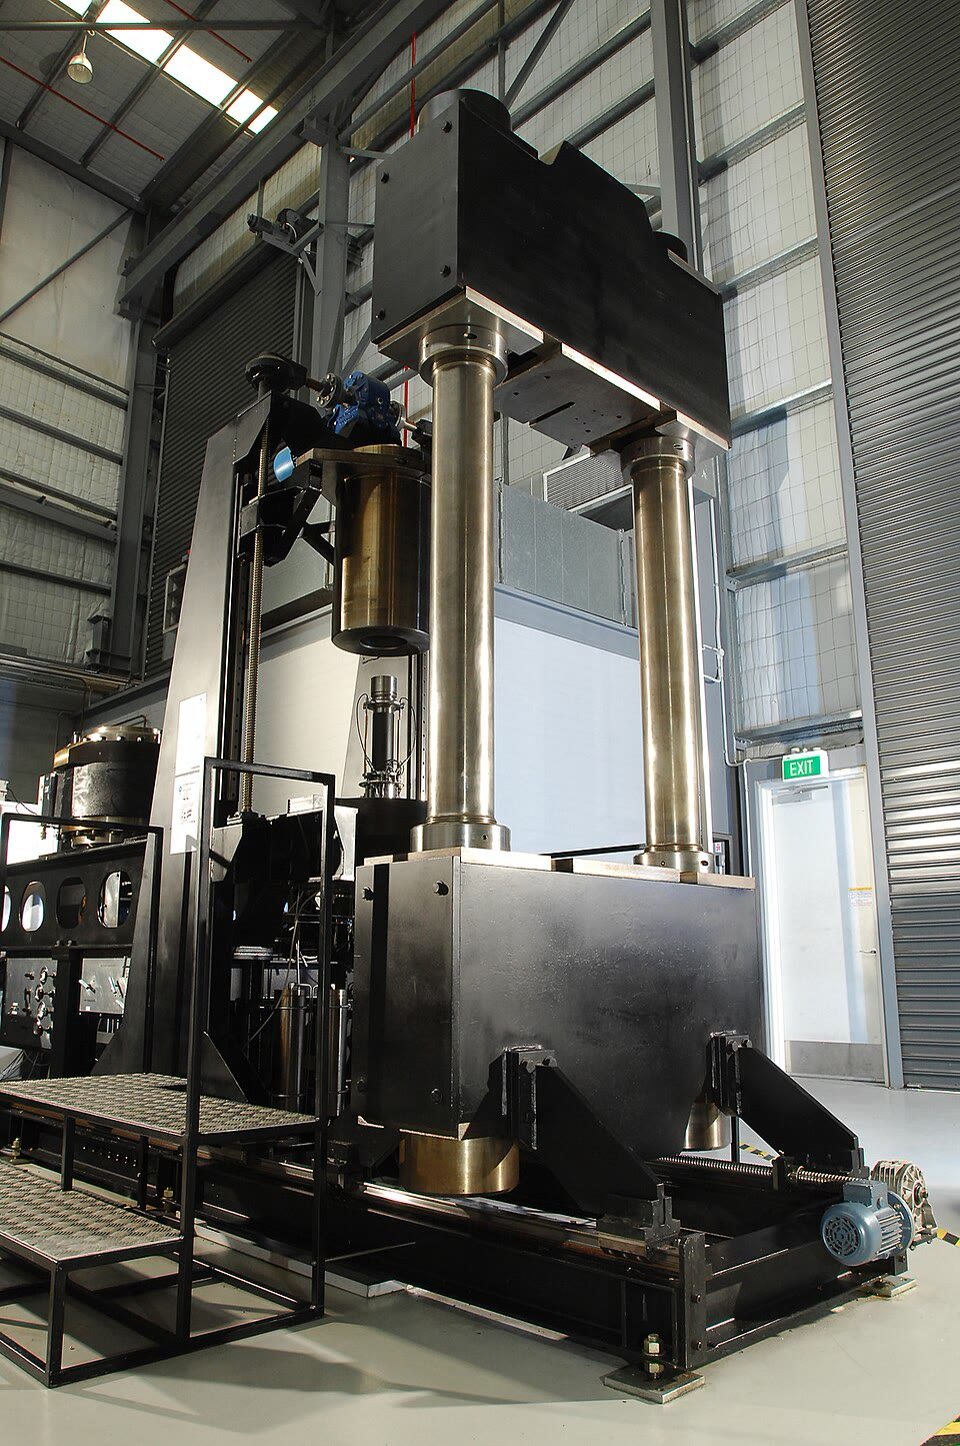
\includegraphics[width=\linewidth]{images/book3/b1-triaxial-cell.jpg}

{\scriptsize A high-pressure triaxial cell for measuring the strength of rock
(Darryl Peroni, CSIRO, CC BY 3.0).}
% ledger: commons:csiro-triaxial
\end{minipage}
\end{inthelab}

\section{The strength of the lithosphere}\label{sec:b1:stress-strain-rheology:envelope}

At every depth the \omterm{def:b1:layered-earth:lithosphere}{lithosphere} can fail in two ways: by sliding on faults,
with a strength that grows with the effective pressure, or by creep, with a
strength that falls as it gets hotter. It deforms in whichever way needs the
smaller stress.

\begin{definition}[Strength envelope, brittle--ductile transition, seismogenic layer]\label{def:b1:stress-strain-rheology:strength-envelope}
The \emph{strength envelope}\index{strength envelope} of the \omterm{def:b1:layered-earth:lithosphere}{lithosphere} is
the curve, against depth, of the largest \omterm{def:b1:stress-strain-rheology:principal}{differential stress} it can bear at a
given strain rate: at each depth, the smaller of the frictional strength and
the creep strength. The \emph{brittle--ductile transition}\index{brittle--ductile
transition} is the depth at which the two are equal: above it the rock
deforms by faulting, below it by creep. The \emph{seismogenic
layer}\index{seismogenic layer} is the range of depths in which most
earthquakes start.
\end{definition}

\begin{proposition}[Frictional strength with depth]\label{prop:b1:stress-strain-rheology:brittle-gradient}
In a layer of density $\rho$ with a hydrostatic pore pressure, one principal
stress vertical, faults of every orientation and no \omterm{def:b1:stress-strain-rheology:coulomb}{cohesion}, sliding with
friction $\mu$ starts at the \omterm{def:b1:stress-strain-rheology:principal}{differential stress}
\begin{align*}
  \sigma_1 - \sigma_3 &= \frac{2\mu}{\sqrt{1+\mu^2} + \mu}\,\rho g z(1-\lambda)
  && \text{if $\sigma_v = \sigma_1$}, \\
  \sigma_1 - \sigma_3 &= \frac{2\mu}{\sqrt{1+\mu^2} - \mu}\,\rho g z(1-\lambda)
  && \text{if $\sigma_v = \sigma_3$},
\end{align*}
with $\lambda = \rho_w/\rho$: the first case gives normal faults, the second
thrusts.
\end{proposition}

\begin{proof}
The vertical \omterm{def:b1:stress-strain-rheology:lithostatic}{effective stress} is $S = \rho g z - \rho_w g z = \rho g z(1-\lambda)$.
With $C = 0$ and $k = \sqrt{1+\mu^2}$, \cref{thm:b1:stress-strain-rheology:failure-angle}
says that a fault slips when $r = \mu c'/k$, with $r$ the radius and $c'$ the
centre of the effective Mohr circle. If $\sigma_v = \sigma_1$, then
$\sigma_1' = S$ and $c' = S - r$, so $rk = \mu S - \mu r$ and
$r = \mu S/(k+\mu)$. If $\sigma_v = \sigma_3$, then $c' = S + r$ and
$r = \mu S/(k-\mu)$. The \omterm{def:b1:stress-strain-rheology:principal}{differential stress} is $2r$.
\end{proof}

With $\mu = 0.85$ and $\rho = \qty{2700}{kg.m^{-3}}$, $S$ grows by
\qty{16.7}{MPa} per kilometre and the frictional strength by
\qty{13.1}{MPa} per kilometre under \omterm{def:b1:stress-strain-rheology:strain}{extension} and \qty{61.3}{MPa} per
kilometre under compression, nearly five times more: a \omterm{def:b1:layered-earth:layers}{crust} is far easier to
pull apart than to push together. Beyond an effective \omterm{def:b1:stress-strain-rheology:stress}{normal stress} of
\qty{200}{MPa} the upper branch of \omterm{prop:b1:stress-strain-rheology:byerlee}{Byerlee's law} takes over, and the slope
falls, in compression, to about \qty{35}{MPa} per kilometre.
% computed in figdata/bachelor-1/strength_envelope.py (tested); ledger: byerlee:1975

\begin{omfigure}
\begin{tikzpicture}
\pgfplotsset{envaxis/.style={omrecord, omdepth, scale only axis, width=5.6cm, height=7.2cm,
  xmin=-1000, xmax=2500, ymin=0, ymax=80, xtick={-1000,0,1000,2000},
  ytick={0,10,...,80}, unbounded coords=jump,
  xlabel={differential stress $\sigma_1-\sigma_3$ (MPa)},
  tick label style={font=\scriptsize}, label style={font=\small},
  scaled x ticks=false, xticklabel style={/pgf/number format/.cd, 1000 sep={\,}}}}
% computed in figdata/bachelor-1/strength_envelope.py; ledger: byerlee:1975, lopez:flow-laws, codata:R, prem:moho-average
\begin{axis}[envaxis, name=cont, ylabel={depth (km)}, title={\small (a) continent, \qty{55}{mW.m^{-2}}}]
\addplot[fill=omLithGranite!45, draw=none] table[x=x, y=depth] {figdata/out/bachelor-1-strength_envelope-continental-outline.dat};
\addplot[omThm, line width=0.5pt, restrict x to domain=-1:2450] table[x=thrust, y=depth] {figdata/out/bachelor-1-strength_envelope-continental.dat};
\addplot[omThm, line width=0.5pt, restrict x to domain=-2450:1] table[x expr=-\thisrow{normal}, y=depth] {figdata/out/bachelor-1-strength_envelope-continental.dat};
\addplot[omDef, line width=0.5pt, restrict x to domain=-1:2450] table[x=ductile, y=depth] {figdata/out/bachelor-1-strength_envelope-continental.dat};
\addplot[omDef, line width=0.5pt, restrict x to domain=-2450:1] table[x expr=-\thisrow{ductile}, y=depth] {figdata/out/bachelor-1-strength_envelope-continental.dat};
\addplot[black, line width=1.0pt] table[x=x, y=depth] {figdata/out/bachelor-1-strength_envelope-continental-outline.dat};
\draw[black!60, dashed] (axis cs:-1000,35) -- (axis cs:2500,35);
\node[font=\scriptsize, anchor=south east] at (axis cs:2480,35) {Moho};
\draw[black, densely dotted] (axis cs:0,0) -- (axis cs:0,80);
\draw[black!70] (axis cs:660,13.7) -- (axis cs:1700,18) node[anchor=north, font=\scriptsize, align=center, text=black] {transition\\ \qty{14}{km}};
\draw[black!70] (axis cs:1870,44.6) -- (axis cs:1950,53) node[anchor=north, font=\scriptsize, align=center, text=black] {mantle\\ transition};
\node[font=\scriptsize, anchor=north, omThm] at (axis cs:1500,3) {compression};
\node[font=\scriptsize, anchor=north, omThm] at (axis cs:-560,3) {extension};
\node[font=\scriptsize, anchor=west, omDef] at (axis cs:40,31) {wet quartz};
\node[font=\scriptsize, anchor=west, omDef] at (axis cs:300,66) {dry olivine};
\end{axis}
\begin{axis}[envaxis, at={(cont.east)}, anchor=west, xshift=0.6cm, yticklabels={}, title={\small (b) ocean floor \qty{60}{Myr} old}]
\addplot[fill=omLithBasalt!45, draw=none] table[x=x, y=depth] {figdata/out/bachelor-1-strength_envelope-oceanic-outline.dat};
\addplot[omThm, line width=0.5pt, restrict x to domain=-1:2450] table[x=thrust, y=depth] {figdata/out/bachelor-1-strength_envelope-oceanic.dat};
\addplot[omThm, line width=0.5pt, restrict x to domain=-2450:1] table[x expr=-\thisrow{normal}, y=depth] {figdata/out/bachelor-1-strength_envelope-oceanic.dat};
\addplot[omDef, line width=0.5pt, restrict x to domain=-1:2450] table[x=ductile, y=depth] {figdata/out/bachelor-1-strength_envelope-oceanic.dat};
\addplot[omDef, line width=0.5pt, restrict x to domain=-2450:1] table[x expr=-\thisrow{ductile}, y=depth] {figdata/out/bachelor-1-strength_envelope-oceanic.dat};
\addplot[black, line width=1.0pt] table[x=x, y=depth] {figdata/out/bachelor-1-strength_envelope-oceanic-outline.dat};
\draw[black, densely dotted] (axis cs:0,0) -- (axis cs:0,80);
\draw[black!70] (axis cs:2003,38.2) -- (axis cs:1900,50) node[anchor=north, font=\scriptsize, align=center, text=black] {transition\\ \qty{38}{km}};
\node[font=\scriptsize, anchor=west, omDef] at (axis cs:300,66) {dry olivine};
\end{axis}
\end{tikzpicture}
\par\smallskip{\small \omterm{def:b1:stress-strain-rheology:strength-envelope}{Strength envelopes} at the strain rate
\qty{e-15}{s^{-1}}. Red: frictional strength from \omterm{prop:b1:stress-strain-rheology:byerlee}{Byerlee's law} with a
hydrostatic pore pressure, for compression (thrust faulting, right) and
\omterm{def:b1:stress-strain-rheology:strain}{extension} (normal faulting, left, drawn as negative); blue: the creep strength
of wet quartzite in the continental \omterm{def:b1:layered-earth:layers}{crust} and of dry \omterm{def:b1:rock-forming-minerals:groups}{olivine} in the \omterm{def:b1:layered-earth:layers}{mantle};
black outline and shading: the strength, the smaller of the two at each
depth. (a) A continent with a surface \omterm{def:b1:heat-budget:heat-flow}{heat flow} of \qty{55}{mW.m^{-2}} and a
\omterm{def:b1:layered-earth:layers}{crust} \qty{35}{km} thick: strong upper \omterm{def:b1:layered-earth:layers}{crust}, weak lower \omterm{def:b1:layered-earth:layers}{crust}, strong
uppermost \omterm{def:b1:layered-earth:layers}{mantle}. (b) Ocean floor \qty{60}{Myr} old: a single strong layer,
\qty{38}{km} thick in compression.}
\label{fig:b1:stress-strain-rheology:envelope}
\end{omfigure}

The figure above puts the two strengths together
for two \omterm{def:b1:layered-earth:lithosphere}{lithospheres}. The continent has the \omterm{def:b1:heat-budget:geotherm}{geotherm} of
\cref{ch:b1:heat-budget} with a surface \omterm{def:b1:heat-budget:heat-flow}{heat flow} of \qty{55}{mW.m^{-2}}, a
\omterm{def:b1:layered-earth:layers}{crust} of wet quartzite \qty{35}{km} thick, and dry \omterm{def:b1:rock-forming-minerals:groups}{olivine} below; the ocean
floor is \qty{60}{Myr} old, with the half-space \omterm{def:b1:heat-budget:geotherm}{geotherm} of the same chapter,
and \omterm{def:b1:rock-forming-minerals:groups}{olivine} from the sea floor down. The strain rate is
\qty{e-15}{s^{-1}}. The \qty{35}{km} is the average depth of the \omterm{def:b1:layered-earth:discontinuity}{Moho} under
the continents in the \omterm{def:b1:layered-earth:reference-model}{reference Earth model} of \cref{ch:b1:layered-earth}.
% ledger: prem:moho-average

Under the continent the \omterm{def:b1:stress-strain-rheology:strength-envelope}{brittle--ductile transition} falls at \qty{13.7}{km}
in compression, at \qty{249}{\degreeCelsius}, and at \qty{17.1}{km} in
\omterm{def:b1:stress-strain-rheology:strain}{extension}. A warmer \omterm{def:b1:layered-earth:layers}{crust} would bring it up, a colder one push it down,
since the creep law depends on the temperature alone at a given stress. The
transition is the strongest level of the \omterm{def:b1:layered-earth:layers}{crust}.
Below it the strength collapses: at the \omterm{def:b1:layered-earth:discontinuity}{Moho}, at \qty{527}{\degreeCelsius},
quartzite flows under \qty{7.6}{MPa}, while \omterm{def:b1:rock-forming-minerals:groups}{olivine} at the same temperature
would need some \qty{30000}{MPa}, so far beyond the frictional strength that
the top of the \omterm{def:b1:layered-earth:layers}{mantle} is brittle again. A second transition follows at
\qty{44.6}{km} in compression. The lower \omterm{def:b1:layered-earth:layers}{crust} of this model is a soft layer
between two strong ones: the ``jelly sandwich''. Under the ocean the whole
\omterm{def:b1:layered-earth:lithosphere}{lithosphere} is \omterm{def:b1:rock-forming-minerals:groups}{olivine}, and the strength grows down to a single transition at
\qty{38.2}{km}, at \qty{641}{\degreeCelsius}.
% computed in figdata/bachelor-1/strength_envelope.py (tested)

The earthquakes agree with the oceanic envelope: inside the oceanic plates,
they reach depths where the temperature is
\qtyrange{600}{800}{\degreeCelsius}, close to the \qty{641}{\degreeCelsius}
of the model's single transition. Deeper earthquakes occur only where one
plate sinks under another, down to more than \qty{700}{km}
(\cref{ch:b1:active-margins}).
% ledger: jackson:jelly, usgs:deepest

The continental \omterm{def:b1:layered-earth:layers}{mantle} is where the picture is disputed. For about twenty
years the jelly sandwich was the prevailing view, built on laboratory
measurements of dry \omterm{def:b1:rock-forming-minerals:groups}{olivine} and on a few earthquakes thought to lie beneath
the \omterm{def:b1:layered-earth:discontinuity}{Moho}. In 2002 James Jackson argued that it should be abandoned: better
depths showed that earthquakes in the continents are confined to a single
layer, usually the upper \omterm{def:b1:layered-earth:layers}{crust}, sometimes the whole \omterm{def:b1:layered-earth:layers}{crust}, with no convincing
earthquakes in the \omterm{def:b1:layered-earth:layers}{mantle} beneath, even where the \omterm{def:b1:layered-earth:discontinuity}{Moho} is only
\qtyrange{300}{500}{\degreeCelsius}. Small amounts of water, a few parts per
million in \omterm{def:b1:rock-forming-minerals:groups}{olivine}, are enough to weaken it dramatically, and the continental
\omterm{def:b1:layered-earth:layers}{mantle} may well hold that much; the strength of the continents would then lie
mostly in their \omterm{def:b1:layered-earth:layers}{crust}. The two views draw different envelopes from the same
laws, with dry or wet \omterm{def:b1:rock-forming-minerals:groups}{olivine} below the \omterm{def:b1:layered-earth:discontinuity}{Moho}.
% ledger: jackson:jelly
Whichever is right, an envelope is a bound and not a measurement: the
laboratory laws are extrapolated over many orders of magnitude of strain rate,
and the peak stresses it shows, more than a gigapascal, are far above the
\qtyrange{1}{10}{MPa} that earthquakes are seen to release.
% ledger: jackson:jelly

\section{Exercises}

\begin{exercise}[$\star$]\label{exo:b1:stress-strain-rheology:1}
Take a \omterm{def:b1:layered-earth:layers}{crust} of density \qty{2700}{kg.m^{-3}} and $g = \qty{9.81}{m.s^{-2}}$.
At a depth of \qty{10}{km}, compute (a) the vertical stress, (b) the
hydrostatic pore pressure, (c) the vertical \omterm{def:b1:stress-strain-rheology:lithostatic}{effective stress} and the
pore-pressure ratio $\lambda$.
\end{exercise}

\begin{exercise}[$\star$]\label{exo:b1:stress-strain-rheology:2}
(a) A bed \qty{10}{km} long is stretched to \qty{13}{km}: give its \omterm{def:b1:stress-strain-rheology:strain}{extension}
and its \omterm{def:b1:stress-strain-rheology:strain}{stretch}. (b) Another, \qty{10}{km} long, is shortened to \qty{7}{km}.
(c) Two lines of a rock that were perpendicular now make an angle of
\ang{60}: what are the angular shear and the \omterm{def:b1:stress-strain-rheology:strain}{shear strain}?
\end{exercise}

\begin{exercise}[$\star$]\label{exo:b1:stress-strain-rheology:3}
At a point, $\sigma_1 = \qty{100}{MPa}$ and $\sigma_3 = \qty{40}{MPa}$.
(a) Draw the Mohr circle. (b) What is the largest shear stress, on which
planes does it act, and what \omterm{def:b1:stress-strain-rheology:stress}{normal stress} acts on them? (c) Compute $\sigma_n$
and $\tau$ on the plane whose normal makes \ang{30} with $\sigma_1$.
\end{exercise}

\begin{exercise}[$\star$]\label{exo:b1:stress-strain-rheology:4}
A rock has the \omterm{def:b1:stress-strain-rheology:coulomb}{cohesion} \qty{10}{MPa} and the \omterm{def:b1:stress-strain-rheology:coulomb}{angle of internal friction}
\ang{30}. (a) At what angle to $\sigma_1$ does it break, and what angle do the
two possible fracture planes make with each other? (b) With
$\sigma_3' = \qty{20}{MPa}$, what effective $\sigma_1'$ breaks it?
\end{exercise}

\begin{exercise}[$\star\star$]\label{exo:b1:stress-strain-rheology:5}
In the axes $x$ (horizontal) and $y$ (vertical), $\sigma_{xx} = \qty{60}{MPa}$,
$\sigma_{yy} = \qty{20}{MPa}$ and $\sigma_{xy} = \qty{15}{MPa}$. (a) Compute the
\omterm{def:b1:stress-strain-rheology:principal}{principal stresses} and the angle $\theta_p$. (b) Check with
\cref{prop:b1:stress-strain-rheology:transformation} that the plane of normal
$\theta_p$ carries no shear stress and the \omterm{def:b1:stress-strain-rheology:stress}{normal stress} $\sigma_1$. (c) What is
the largest shear stress at this point?
\end{exercise}

\begin{exercise}[$\star\star$]\label{exo:b1:stress-strain-rheology:6}
A shear zone has deformed its rock by a \omterm{def:b1:stress-strain-rheology:shear-types}{simple shear} $\gamma = 2$. (a) Compute
the principal \omterm{def:b1:stress-strain-rheology:strain}{stretches} and the angle of the long axis of the \omterm{def:b1:stress-strain-rheology:strain-ellipse}{strain ellipse}
to the shear direction. (b) Check that the area has not changed. (c) A line of
material was at \ang{45} to the shear direction, rising in the sense of the
shear: where does it lie now, and what is its \omterm{def:b1:stress-strain-rheology:strain}{stretch}? Compare with (a).
\end{exercise}

\begin{exercise}[$\star\star$]\label{exo:b1:stress-strain-rheology:7}
In a shear zone \qty{200}{m} thick, small round spots in a slate have become
ellipses with axes in the ratio 4 to 1. Assume a \omterm{def:b1:stress-strain-rheology:shear-types}{simple shear}, with no change
of area. (a) Find $S_1$, $S_2$ and $\gamma$. (b) At what angle to the walls of
the zone should the long axes lie? (c) How far has one wall moved past the
other?
\end{exercise}

\begin{exercise}[$\star\star$]\label{exo:b1:stress-strain-rheology:8}
A fault at a depth of \qty{3}{km}, in \omterm{def:b1:layered-earth:layers}{crust} of density \qty{2700}{kg.m^{-3}},
carries the \omterm{def:b1:stress-strain-rheology:stress}{normal stress} \qty{70}{MPa} and the shear stress \qty{30}{MPa}.
(a) With a hydrostatic pore pressure, does it slip according to \omterm{prop:b1:stress-strain-rheology:byerlee}{Byerlee's
law}? (b) And if the pores are sealed and $\lambda = 0.6$? (c) Find the value
of $\lambda$ at which it starts to slip.
\end{exercise}

\begin{exercise}[$\star\star$]\label{exo:b1:stress-strain-rheology:9}
Use the creep law of wet quartzite (\cref{prop:b1:stress-strain-rheology:creep}).
(a) By what factor must the stress rise to make it flow ten times faster?
(b) By what factor does its strength fall between \qty{400}{\degreeCelsius}
and \qty{500}{\degreeCelsius}, at the same rate and with $V = 0$? (c) Explain
with these two results why the depth of the \omterm{def:b1:stress-strain-rheology:strength-envelope}{brittle--ductile transition}
depends much more on the \omterm{def:b1:heat-budget:geotherm}{geotherm} than on the strain rate.
\end{exercise}

\begin{exercise}[$\star\star\star$]\label{exo:b1:stress-strain-rheology:10}
Where the vertical stress is $\sigma_2$, faults are strike-slip. Assume that
the vertical \omterm{def:b1:stress-strain-rheology:lithostatic}{effective stress} is then the mean $(\sigma_1' + \sigma_3')/2$.
(a) Show that sliding with friction $\mu$ and no \omterm{def:b1:stress-strain-rheology:coulomb}{cohesion} starts at
$\sigma_1 - \sigma_3 = 2\mu\,\rho g z(1-\lambda)/\sqrt{1+\mu^2}$. (b) Compute
the slope in megapascals per kilometre for $\mu = 0.85$ and
$\rho = \qty{2700}{kg.m^{-3}}$, and place it between the slopes of normal and
thrust faulting. (c) Express each of the three slopes as a multiple of the
vertical \omterm{def:b1:stress-strain-rheology:lithostatic}{effective stress}.
\end{exercise}

\begin{exercise}[$\star\star\star$]\label{exo:b1:stress-strain-rheology:11}
Model the oceanic \omterm{def:b1:layered-earth:lithosphere}{lithosphere} \qty{60}{Myr} old as a half-space cooled from
\qty{1350}{\degreeCelsius}, with a surface at \qty{0}{\degreeCelsius} and
$\kappa = \qty{e-6}{m^2.s^{-1}}$: $T = \num{1350}\operatorname{erf}\bigl(z/(2\sqrt{\kappa t})\bigr)$.
(a) Compute $2\sqrt{\kappa t}$. (b) Find the depths of the
\qty{600}{\degreeCelsius} and \qty{800}{\degreeCelsius} isotherms. (c) Earthquakes
inside the oceanic plates reach the depths where the temperature is
\qtyrange{600}{800}{\degreeCelsius}. Compare with the \omterm{def:b1:stress-strain-rheology:strength-envelope}{brittle--ductile
transition} in the oceanic \omterm{def:b1:stress-strain-rheology:strength-envelope}{strength envelope} of this chapter, at
\qty{38.2}{km} and \qty{641}{\degreeCelsius}.
% ledger: jackson:jelly
\end{exercise}

\begin{exercise}[$\star\star\star$]\label{exo:b1:stress-strain-rheology:12}
A rock is crossed by fractures of every orientation, all containing the
direction of $\sigma_2$, with no \omterm{def:b1:stress-strain-rheology:coulomb}{cohesion} and friction 0.85. The effective
\omterm{def:b1:stress-strain-rheology:principal}{principal stresses} are $\sigma_1' = \qty{110}{MPa}$ and
$\sigma_3' = \qty{20}{MPa}$. (a) Show that some fractures slip. (b) Find the
range of the angle between the slipping fractures and $\sigma_1$. Which one is
in the middle of the range? (c) Down to what value of $\sigma_1'$, with
$\sigma_3'$ fixed, does at least one fracture still slip?
\end{exercise}

\section{Problem: Will the fault slip?}

\begin{problem}[{Weekend problem --- the stress on a normal fault at a depth
of five kilometres, its safety margin, and the rise of pore pressure that
would make it slip}]
\label{pb:b1:stress-strain-rheology:1}
% values: calc/ch16.py; ledger: byerlee:1975, hb81:denver
A fault \omterm{def:b1:geological-maps:attitude}{strikes} north--south and \omterm{def:b1:geological-maps:attitude}{dips} \ang{60} to the east. A disposal well
reaches it at a depth of \qty{5.00}{km}, in \omterm{def:b1:layered-earth:layers}{crust} of density
\qty{2700}{kg.m^{-3}} whose pores connect to the surface. A measurement in the
well gives the horizontal stress perpendicular to the fault,
\qty{75.0}{MPa}; the horizontal stress along the \omterm{def:b1:geological-maps:attitude}{strike} lies between it and
the vertical stress, so the problem is two-dimensional in the vertical plane
east--west. Take $g = \qty{9.81}{m.s^{-2}}$, water of density
\qty{1000}{kg.m^{-3}} and \omterm{prop:b1:stress-strain-rheology:byerlee}{Byerlee's law}. Give stresses to
\qty{0.01}{MPa}.

\medskip
\noindent\textbf{Part I --- The state of stress.}
\begin{enumerate}
  \item Compute the vertical stress at the depth of the fault.
  \item Compute the hydrostatic pore pressure there, and the ratio $\lambda$.
  \item Which of the two stresses is $\sigma_1$ and which $\sigma_3$? What kind
        of fault does this state of stress drive?
  \item Compute the \omterm{def:b1:stress-strain-rheology:principal}{differential stress}, the centre and the radius of the
        Mohr circle.
  \item Compute the effective \omterm{def:b1:stress-strain-rheology:principal}{principal stresses} and the centre of the
        effective circle.
  \item With $x$ horizontal to the east and $y$ vertical, write the three
        components $\sigma_{xx}$, $\sigma_{yy}$, $\sigma_{xy}$. Why is
        $\sigma_{xy}$ zero?
\end{enumerate}

\medskip
\noindent\textbf{Part II --- The stresses on the fault.}
\begin{enumerate}[resume]
  \item Give the unit normal to the fault in the axes of question 6, and the
        angle $\theta$ between it and $\sigma_1$.
  \item Compute $\sigma_n$ and $\tau$ on the fault with
        \cref{prop:b1:stress-strain-rheology:transformation}.
  \item Check both values with Mohr's circle: at what angle from the $\sigma_1$
        end does the fault lie?
  \item Compute the effective \omterm{def:b1:stress-strain-rheology:stress}{normal stress} on the fault.
  \item Compute the ratio $\tau/\sigma_n'$ and compare it with 0.85.
  \item What shear stress would make the fault slip under the present
        effective \omterm{def:b1:stress-strain-rheology:stress}{normal stress}? By how many megapascals is it short?
\end{enumerate}

\medskip
\noindent\textbf{Part III --- Mohr's circle and Byerlee's law.}
\begin{enumerate}[resume]
  \item Draw the effective Mohr circle and Byerlee's line to scale.
  \item Compute the distance from the centre of the circle to the line and
        compare it with the radius. Can any plane through the rock slip?
  \item Which plane would slip first? Give its angle to $\sigma_1$ and its \omterm{def:b1:geological-maps:attitude}{dip}.
  \item With \cref{prop:b1:stress-strain-rheology:brittle-gradient}, compute the
        \omterm{def:b1:stress-strain-rheology:principal}{differential stress} at which normal faults slip at this depth, and
        check it against the slope of \qty{13.1}{MPa} per kilometre.
  \item How low would the horizontal stress have to fall for the best-oriented
        plane to slip?
  \item How low for the fault of the problem to slip? Explain why it is
        lower.
\end{enumerate}

\medskip
\noindent\textbf{Part IV --- Injection.}
\begin{enumerate}[resume]
  \item Explain why a rise $\Delta P$ of the pore pressure moves the effective
        circle by $\Delta P$ to the left without changing its radius.
  \item Compute the rise of pore pressure that brings the best-oriented plane
        to slip.
  \item The well is full of water. What extra pressure must the pump apply at
        the wellhead to raise the pore pressure at the fault by that amount?
        How high a column of water is it equivalent to?
  \item If the friction on the fault were 0.6 rather than 0.85, would it be
        slipping already? What does the quiet of the fault say about its
        friction?
  \item At what ratio $\lambda$ does the best-oriented plane slip?
  \item To one decimal, in megapascals, what rise of pore pressure brings this
        fault to slip?
\end{enumerate}
\end{problem}
